\documentclass[a4paper,11pt]{article}
\pagestyle{headings}

\usepackage[utf8]{inputenc}
\usepackage[francais]{babel}
\usepackage{graphicx}
\usepackage[T1]{fontenc}


\title{Projet Algo1 : Sac de noeuds}
\author{Romain DULERY, Aymeric COLLANGE}
\date{\today}

\begin{document}

\maketitle

~\\
\section{Présentation globale du projet}

Le projet consistait à réaliser un algorithme de tracé de nœuds celtiques.
L'objectif intermédiaire était de choisir une structure de donnée adaptée au problème et générer à partir d'un fichier .kn, un squelette de graphe contenant des arêtes et des croix (qui nous permettront  plus tard de tracer les courbes).
Voici, ci-dessous, un exemple de réalisation de ce type de graphe.\\

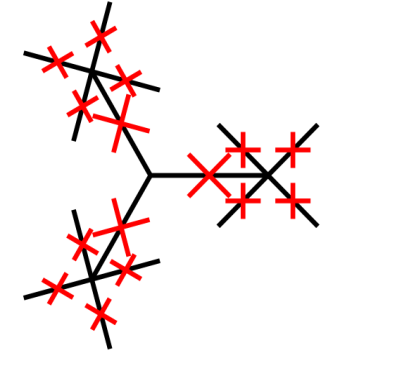
\includegraphics{Banana4.png}
~\\

\section{Choix de la structure de données}

Le nombre de sommets étant connus dès le début de la lecture du fichier et la désignation d'un sommet par son numéro étant intuitive, nous avons donc choisi un tableau de sommet.
Afin de stocker les données nécessaires, plusieurs structures ont été créées. C'est le cas, notamment, de la structure Arete, commune à deux sommets, qui contient le point milieu de l'arête ainsi que la croix (autre structure contenant les quatre points de contrôle pour le tracé futur des courbes).
Ici, seulement des tableaux ont été utilisés car nous n'avons pas jugé utile l'implémentation d'une liste ou d'une pile dans le cadre de ce problème.

\section{Possibilité d'amélioration}

Nous n'avons, malheureusement, pas pu atteindre l'objectif final du projet.
Au niveau des améliorations sur ce qui a été fait, nous n'avons pas adapté la taille de l'image svg à l'entrée.

\end{document}

